\documentclass{article}
\usepackage{tikz}

\begin{document}

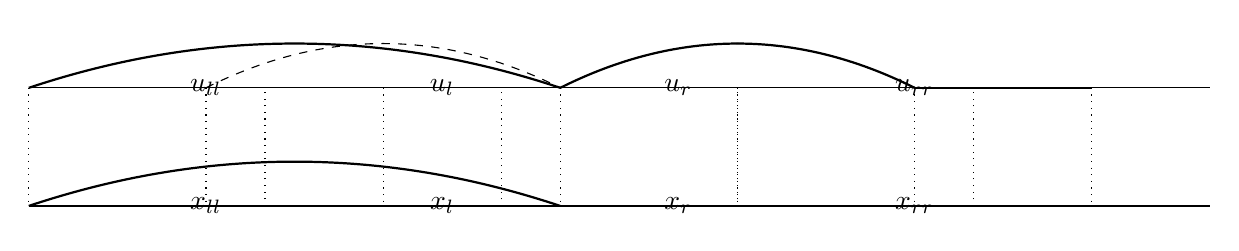
\begin{tikzpicture}[scale=1.5]
    % Draw the horizontal lines
    \draw (0,0) -- (10,0);
    \draw (0,-1) -- (10,-1);
    
    % Draw the vertical dotted lines
    \foreach \x in {2,4,6,8} {
        \draw[dotted] (\x,-1) -- (\x,0);
    }
    
    % Draw the labels for u
    \node at (1.5,0) {$u_{ll}$};
    \node at (3.5,0) {$u_l$};
    \node at (5.5,0) {$u_r$};
    \node at (7.5,0) {$u_{rr}$};
    
    % Draw the labels for x
    \node at (1.5,-1) {$x_{ll}$};
    \node at (3.5,-1) {$x_l$};
    \node at (5.5,-1) {$x_r$};
    \node at (7.5,-1) {$x_{rr}$};
    
    % Draw the solid line for x
    \draw[thick] (0,-1) .. controls (1.5,-0.5) and (3,-0.5) .. (4.5,-1);
    
    % Draw the dashed line for u
    \draw[dashed] (0,0) -- (1.5,0);
    \draw[dashed] (1.5,0) .. controls (2.5,0.5) and (3.5,0.5) .. (4.5,0);
    \draw[dashed] (4.5,0) .. controls (5.5,0.5) and (6.5,0.5) .. (7.5,0);
    \draw[dashed] (7.5,0) -- (9,0);
    
    % Draw the solid line for u
    \draw[thick] (0,0) .. controls (1.5,0.5) and (3,0.5) .. (4.5,0);
    \draw[thick] (4.5,0) .. controls (5.5,0.5) and (6.5,0.5) .. (7.5,0);
    \draw[thick] (7.5,0) -- (9,0);
    
    % Draw the horizontal lines for u
    \draw[dotted] (0,0) -- (0,-1);
    \draw[dotted] (1.5,0) -- (1.5,-1);
    \draw[dotted] (3,0) -- (3,-1);
    \draw[dotted] (4.5,0) -- (4.5,-1);
    \draw[dotted] (6,0) -- (6,-1);
    \draw[dotted] (7.5,0) -- (7.5,-1);
    \draw[dotted] (9,0) -- (9,-1);
\end{tikzpicture}

\end{document}